\documentclass[aspectratio=169]{beamer}
\usepackage{color,amsmath}
\usepackage{subfigure}
\usepackage{booktabs}
\usepackage{framed}
\usepackage{comment}
\usepackage{hyperref}
\usepackage{ulem}

\usepackage{tikz}
\usetikzlibrary{arrows,shapes.arrows,positioning,shapes}
\newcommand\E{\text{E}}
\newcommand\blue[1]{{\color{blue}#1}}
\newcommand\bblue[1]{{\color{blue}\textbf{#1}}}
\newcommand\black[1]{{\color{black}#1}}
\newcommand\white[1]{{\color{white}#1}}
\usepackage{amsmath}

\usepackage{hyperref}
\hypersetup{
    colorlinks=true,
    linkcolor=blue,
    filecolor=magenta,      
    urlcolor=cyan,
}

%\usetheme{default}
%\beamertemplatenavigationsymbolsempty
%\usetikzlibrary{arrows,shapes.arrows,positioning,shapes}
%\usepackage{graphicx}
%\usepackage{hyperref}
%\usepackage{comment}
%\usepackage{ulem}
%
%\newcommand\red[1]{{\color{red}#1}}
%\newcommand\bred[1]{{\color{red}\textbf{#1}}}
%\newcommand\V{\text{V}}
%\renewcommand\P{\text{P}}
%

%%%%%%%%%%%%%%%%%%%%%%%%%%
\title[]{\textcolor{gray}{[Introduction to mass collaboration], [Human computation], [Open call], [Distributed data collection],} \newline [Fragile Families Challenge]}
\author[]{Matthew J. Salganik\\Department of Sociology\\Princeton University}
\date[]{%Summer Institutes in Computational Social Science\\2020
%\vfill
%\begin{flushleft}
%{\scriptsize
%The Summer Institutes in Computational Social Science is supported by grants from the Russell Sage Foundation and the Alfred P. Sloan Foundation.}
%\end{flushleft}
\begin{flushright}

\includegraphics[width=0.1\textwidth]{figures/cc-by.png}
\end{flushright}
}
\begin{document}
%%%%%%%%%%%%%%%%%%%%%%%%%%
\frame{\titlepage}
%%%%%%%%%%%%%%%%%%%%%%%%%%
\begin{frame}

\begin{columns}
\begin{column}{.40\textwidth}
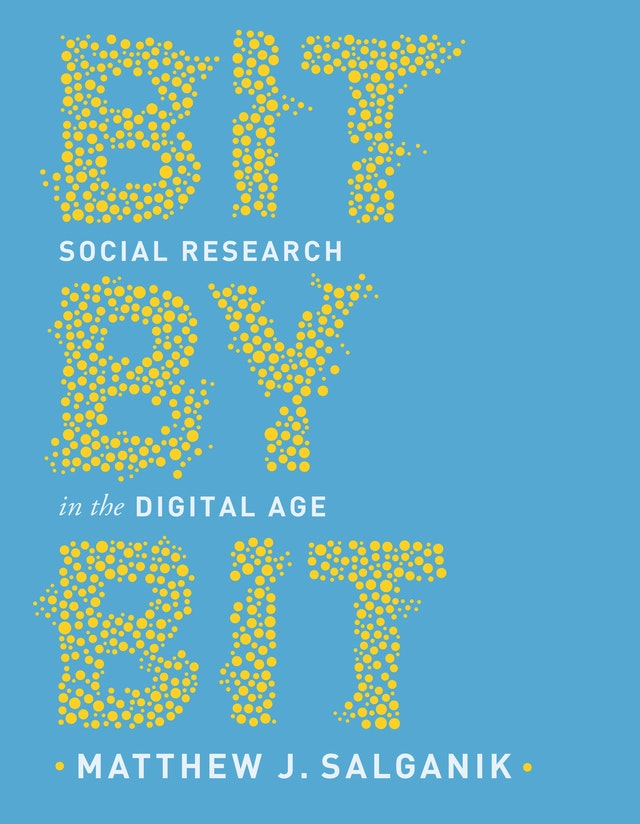
\includegraphics[width=\textwidth]{figures/salganik_bit_2018_cover}
\end{column}%

\hfill%

\begin{column}{.60\textwidth}
1) Introduction \\
2) Observing behavior \\
3) Asking questions \\
4) Running experiments \\
\textcolor{blue}{5) Mass collaboration} \\
6) Ethics \\
7) The future \\
\end{column}%
\end{columns}

\end{frame}
%%%%%%%%%%%%%%%%%%%%%%%%%
\begin{frame}

\begin{center}
\only<1>{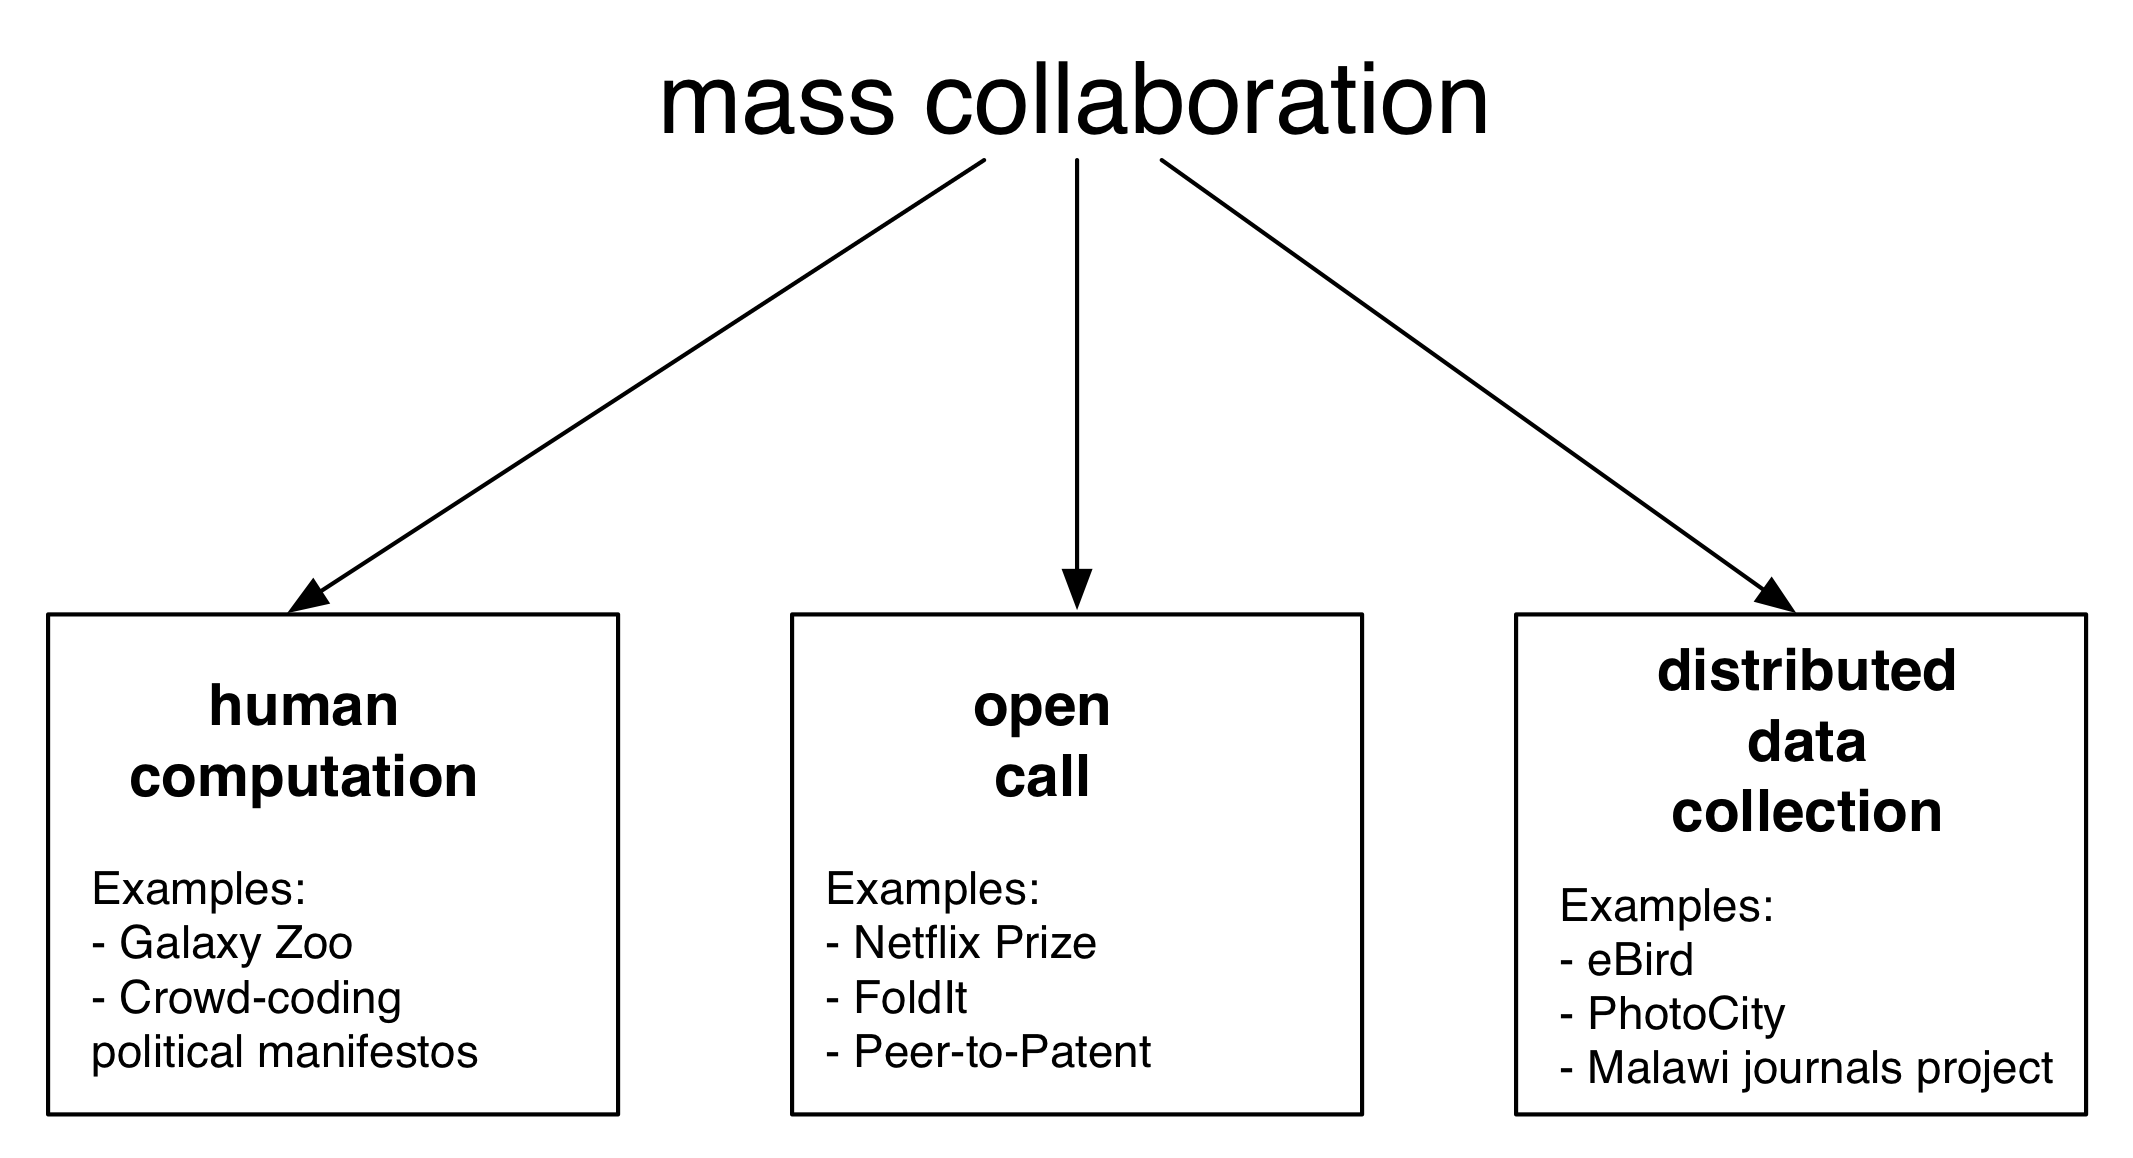
\includegraphics[width=0.9\textwidth]{figures/mass_collaboration_schematic}}
\only<2>{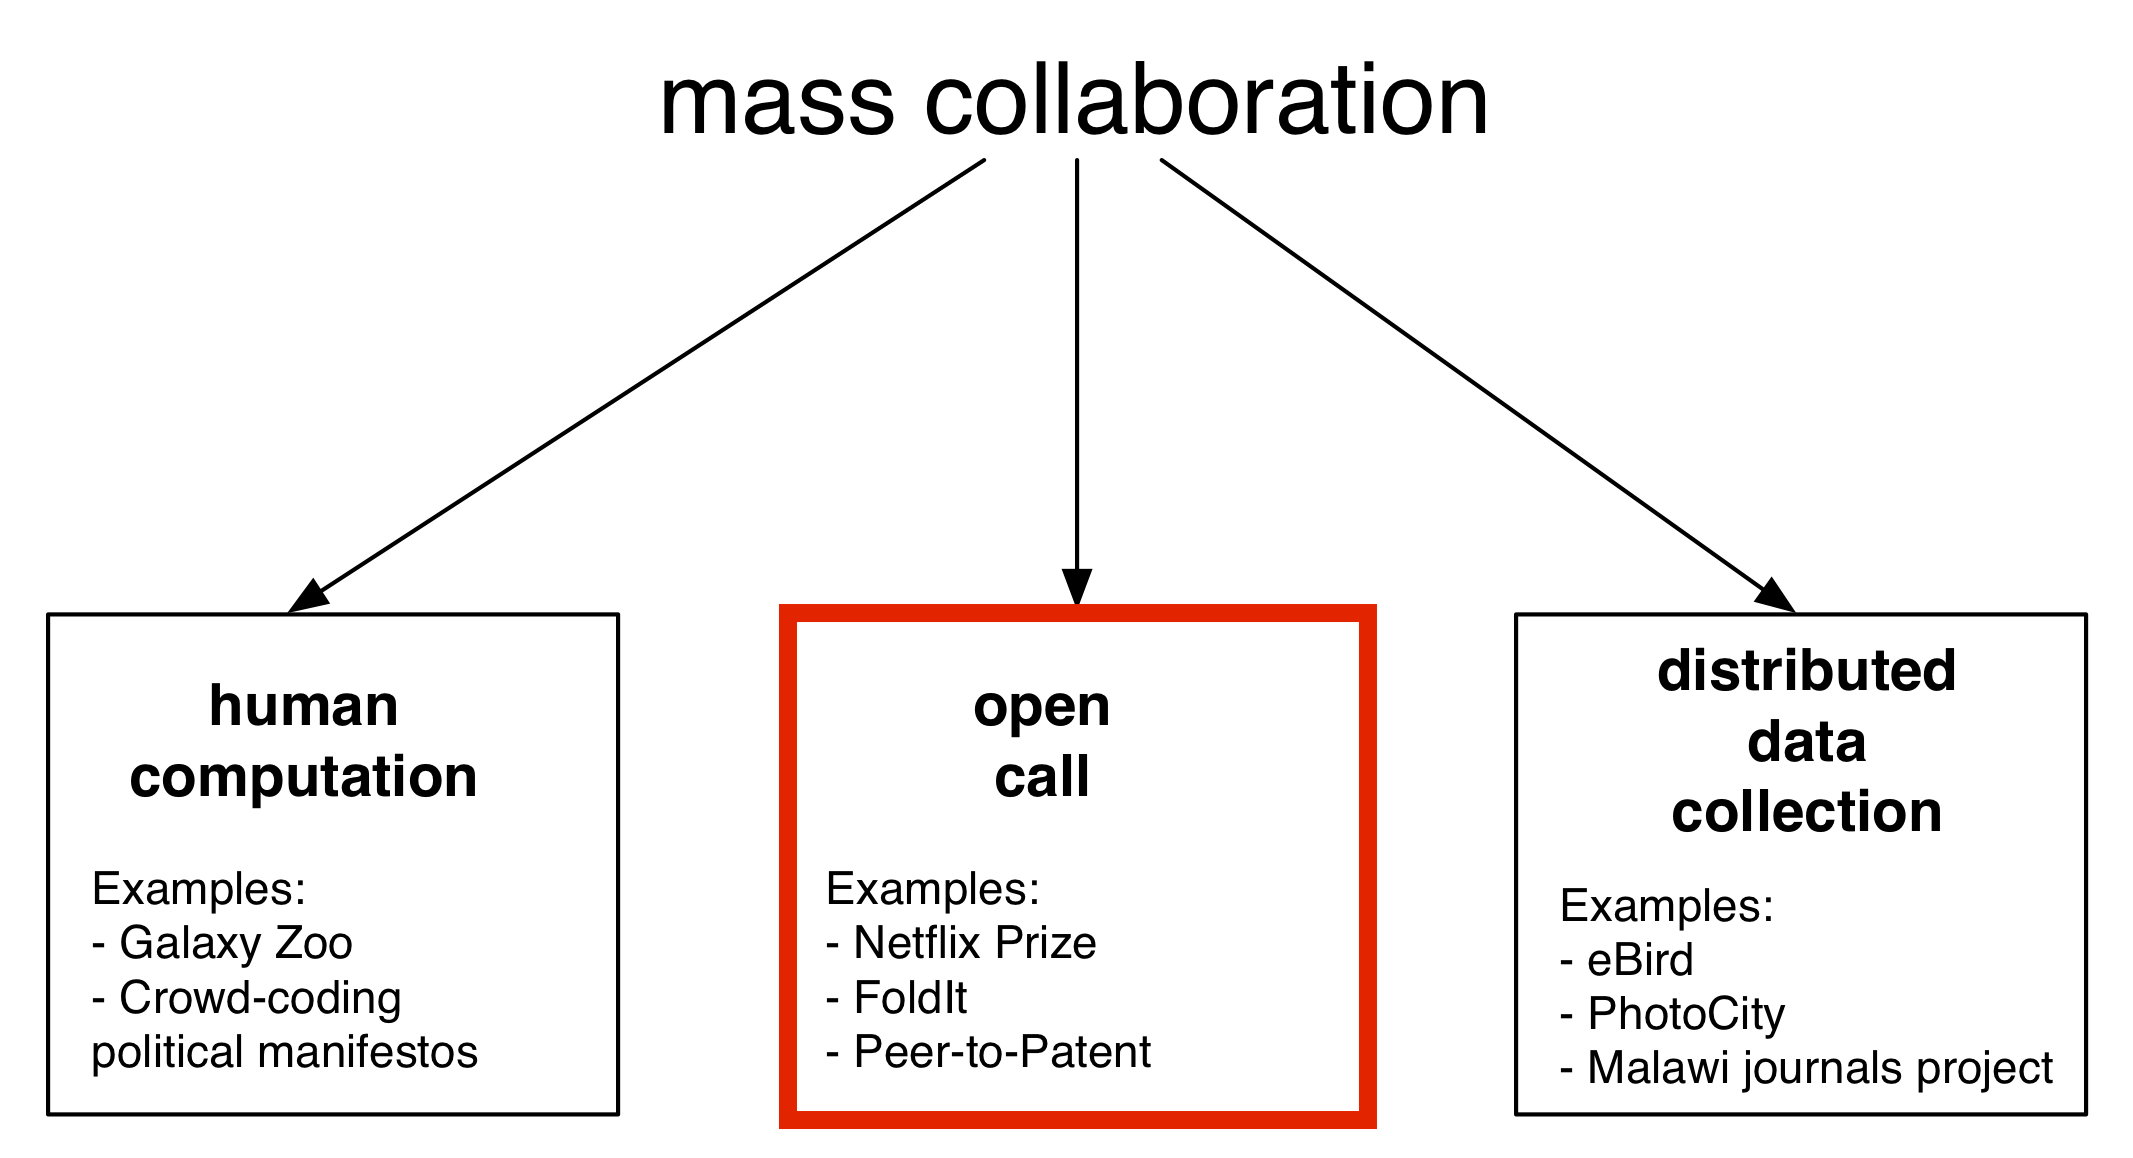
\includegraphics[width=0.9\textwidth]{figures/mass_collaboration_schematic_open_call}}
\end{center}

\vfill
Fig 5.4 (\href{https://www.bitbybitbook.com/}{Salganik 2018})
\end{frame}

%%%%%%%%%%%%%%%%%%%%%%%%%%
\title{Measuring the Predictability of Life Outcomes with a Scientific Mass Collaboration}

\author{{\small Matthew Salganik, Ian Lundberg, Alex Kindel, Sara McLanahan,\\and the participants in the Fragile Families Challenge}}

\institute[]{}
\date{\vfill
\begin{flushleft}{\tiny Funding for FFCWS provided by NICHD (R01HD36916, R01HD39135, R01HD40421) and a consortium of private foundations, including the Robert Wood Johnson Foundation. Funding for FFC provided by the Russell Sage Foundation, NSF, \& the Overdeck Fund. FFC Board of Advisors: Jeanne Brooks-Gunn, Kathryn Edin, Barbara Engelhardt, Irwin Garfinkel, Moritz Hardt, Dean Knox, Nicholas Lemann, Karen Levy, Sara McLanahan, Arvind Narayanan, Timothy Nelson, Matthew Salganik, Brandon Stewart \& Duncan Watts.}
\end{flushleft}
}

%%%%%%%%%%%%%%%%%%%%%%%%%%%%%%
\begin{frame}
  \titlepage
\end{frame}
%%%%%%%%%%%%%%%%%%%%%%%%%%%
\begin{frame}

\begin{center}
\includegraphics[width=0.6\textwidth]{figures/wikipedia_logo}
\end{center}

\end{frame}
%%%%%%%%%%%%%%%%%%%%%%%%%%%
\begin{frame}

\begin{center}
\includegraphics[width=0.9\textwidth]{figures/lander_initial_2001_title}
\end{center}

\vfill
{\tiny \url{http://dx.doi.org/10.1038/35057062}}

\end{frame}
%%%%%%%%%%%%%%%%%%%%%%%%%%
\begin{frame}

\begin{center}
\includegraphics[height=0.9\textheight]{figures/lander_initial_2001_authors}
\end{center}

\end{frame}
%%%%%%%%%%%%%%%%%%%%%%%%%%
\begin{frame}

\begin{center}
\includegraphics[width=\textwidth]{figures/aad_combined_2015_title}
\end{center}

\vfill
{\tiny \url{https://doi.org/10.1103/PhysRevLett.114.191803}}

\end{frame}
%%%%%%%%%%%%%%%%%%%%%%%%%%
\begin{frame}

\begin{center}
\only<1>{\includegraphics[height=\textheight]{figures/aad_combined_2015_authors_01}}%
\only<2>{\includegraphics[height=\textheight]{figures/aad_combined_2015_authors_02}}%
\only<3>{\includegraphics[height=\textheight]{figures/aad_combined_2015_authors_03}}%
\only<4>{\includegraphics[height=\textheight]{figures/aad_combined_2015_authors_04}}%
\only<5>{\includegraphics[height=\textheight]{figures/aad_combined_2015_authors_05}}%
\only<6>{\includegraphics[height=\textheight]{figures/aad_combined_2015_authors_06}}%
\only<7>{\includegraphics[height=\textheight]{figures/aad_combined_2015_authors_07}}%
\only<8>{\includegraphics[height=\textheight]{figures/aad_combined_2015_authors_08}}%
\only<9>{\includegraphics[height=\textheight]{figures/aad_combined_2015_authors_09}}%
\only<10>{\includegraphics[height=\textheight]{figures/aad_combined_2015_authors_10}}%
\only<11>{\includegraphics[height=\textheight]{figures/aad_combined_2015_authors_11}}%
\only<12>{\includegraphics[height=\textheight]{figures/aad_combined_2015_authors_12}}%
\only<13>{\includegraphics<13>[height=\textheight]{figures/aad_combined_2015_authors_13}}%
\only<14>{\includegraphics<14>[height=\textheight]{figures/aad_combined_2015_authors_14}}%
\only<15>{\includegraphics<15>[height=\textheight]{figures/aad_combined_2015_authors_15}}%
\only<16>{\includegraphics<16>[height=\textheight]{figures/aad_combined_2015_authors_16}}%
\only<17>{\includegraphics<17>[height=\textheight]{figures/aad_combined_2015_authors_17}}%
\only<18>{\includegraphics<18>[height=\textheight]{figures/aad_combined_2015_authors_18}}%
\only<19>{\includegraphics<19>[height=\textheight]{figures/aad_combined_2015_authors_19}}%
\only<20>{\includegraphics<20>[height=\textheight]{figures/aad_combined_2015_authors_20}}%
\only<21>{\includegraphics<21>[height=\textheight]{figures/aad_combined_2015_authors_21}}%
\only<22>{\includegraphics<22>[height=\textheight]{figures/aad_combined_2015_authors_22}}%
\only<23>{\includegraphics<23>[height=\textheight]{figures/aad_combined_2015_authors_23}}%
\only<24>{\includegraphics<24>[height=\textheight]{figures/aad_combined_2015_authors_24}}%
\only<25>{\includegraphics<25>[height=\textheight]{figures/aad_combined_2015_authors_25}}
\end{center}

\end{frame}
%%%%%%%%%%%%%%%%%%%%%%%%%
\begin{frame}

\begin{center}

\includegraphics[width=\textwidth]{figures/ffc_masthead}
\Large{Fragile Families Challenge}
\end{center}

\end{frame}
%%%%%%%%%%%%%%%%%%%%%%%%%%%%%%%%
\begin{frame}

Life course researchers have:
\begin{itemize}
\item described social patterns
\item theorized important factors
\item estimated causal effects
\end{itemize}

\pause
\vfill
How well can we predict individual life outcomes?

\end{frame}
%%%%%%%%%%%%%%%%%%%%%%%%%%%%%%%
\begin{frame}

\begin{center}
\LARGE{
$ \hat{y} \quad \& \quad \hat{\beta}$
}
\end{center}

\vfill
\href{https://dx.doi.org/10.1257/jep.31.2.87}{Mullainathan and Spiess (2017)}
\end{frame}
%%%%%%%%%%%%%%%%%%%%%%%%%%
\begin{frame}

We should care about the predictability of social outcomes\pause
\begin{itemize}
\item Scientific reasons \pause
\begin{itemize}
\item Basic social fact \pause
\item Discovery \pause
\end{itemize}
\item Policy reasons
\begin{center}
\includegraphics[width=0.8\textwidth]{figures/hurley_can_2018_title} 
\end{center}
\end{itemize}

\end{frame}
%%%%%%%%%%%%%%%%%%%%%%%%%
\begin{frame}

\begin{center}
\includegraphics[width=\textwidth]{figures/ff_logo}
\end{center}

\begin{itemize}
\item Birth cohort panel study
\item $\approx$ 5,000 children born in 20 U.S. cities with an over-sample of non-marital births
\item Followed from birth through age 15
\item Already used in hundreds of papers and dozens of dissertations
\end{itemize}

\end{frame}
%%%%%%%%%%%%%%%%%%%%%%%%%%%
\begin{frame}

\begin{center}
\only<1>{\includegraphics[width=0.8\textwidth]{figures/ff_design_public_b9}}
\only<2>{\includegraphics[width=0.8\textwidth]{figures/ff_design_public2}}
\end{center}

\end{frame}
%%%%%%%%%%%%%%%%%%%%%%%%%
\begin{frame}

\begin{center}
\includegraphics[width=\textwidth]{figures/ff_design_matrix_ml}
\end{center}

\end{frame}
%%%%%%%%%%%%%%%%%%%%%%%%%
\begin{frame}

\begin{center}
\includegraphics[width=\textwidth]{figures/ffc_design_matrix_ml}
\end{center}

\end{frame}
%%%%%%%%%%%%%%%%%%%%%%%%%
\begin{frame}

Outcomes
\begin{itemize}
\item Child: GPA (continuous), Grit (continuous)
\item Household:  Eviction (binary), Material hardship (continuous)
\item Primary care giver: Job training (binary), Job loss (binary)
\end{itemize}

\end{frame}
%%%%%%%%%%%%%%%%%%%%%%%%%
\begin{frame}

457 researchers applied to participate. Many worked in interdisciplinary teams.
\pause
Using a large, high-quality social science dataset collected since birth and modern machine learning methods, how accurately can we predict outcomes from children, parents, and families?

\begin{equation*}
R^2_{holdout} = 1 - \frac{\sum_{i \in \text{holdout}} (\hat{y}_i - y_i)^2}{\sum_{i \in \text{holdout}} (\bar{y}_{train} - y_i)^2}
\end{equation*}

\end{frame}
%%%%%%%%%%%%%%%%%%%%%%%%%
\begin{frame}

\begin{center}
\only<1>{\includegraphics[width=0.95\textwidth]{figures/RSquared_all_ASA.pdf}}
\only<2>{\includegraphics[width=0.95\textwidth]{figures/RSquared_all_ASA_01.pdf}}
\end{center}

\end{frame}
%%%%%%%%%%%%%%%%%%%%%%
\begin{frame}

\begin{center}
\Large{Is this even better than a benchmark model?}
\end{center}

\end{frame}
%%%%%%%%%%%%%%%%%%%
\begin{frame}

\begin{center}
\only<1>{\includegraphics[width=0.95\textwidth]{figures/RSquared_all_ASA_01.pdf}} %
\only<2>{\includegraphics[width=0.95\textwidth]{figures/RSquared_all_ASA_01_benchmark.pdf}} %
\end{center}

\vfill 

\onslide<2>{Green line: 4 variable regression model}

\end{frame}
%%%%%%%%%%%%%%%%%%%%%%%%%%%
\begin{frame}

\begin{center}
\only<1>{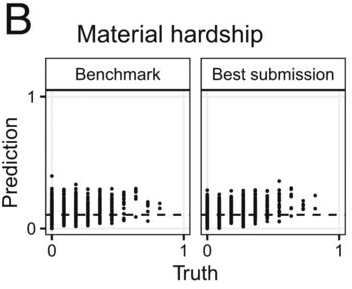
\includegraphics[width=0.6\textwidth]{figures/salganik_measuring_2020_fig3b}} %
\only<2>{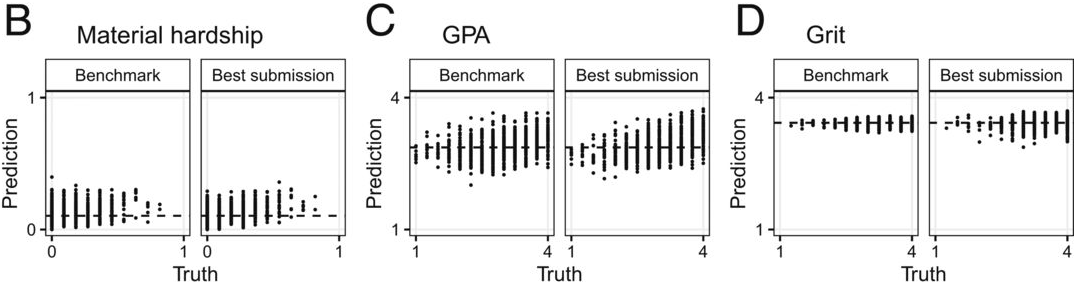
\includegraphics[width=0.9\textwidth]{figures/salganik_measuring_2020_fig3bd}} %
\end{center}

\vfill
Fig 3, \href{https://doi.org/10.1073/pnas.1915006117}{Salganik et al.\ (2020)}
\end{frame}
%%%%%%%%%%%%%%%%%%%%%%%%%%%
\begin{frame}

\begin{center}
\only<1>{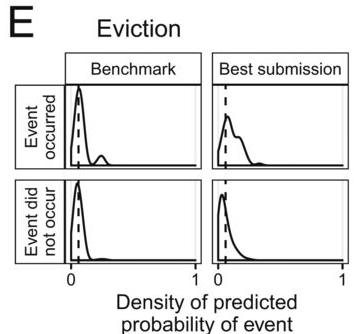
\includegraphics[width=0.6\textwidth]{figures/salganik_measuring_2020_fig3e}} %
\only<2>{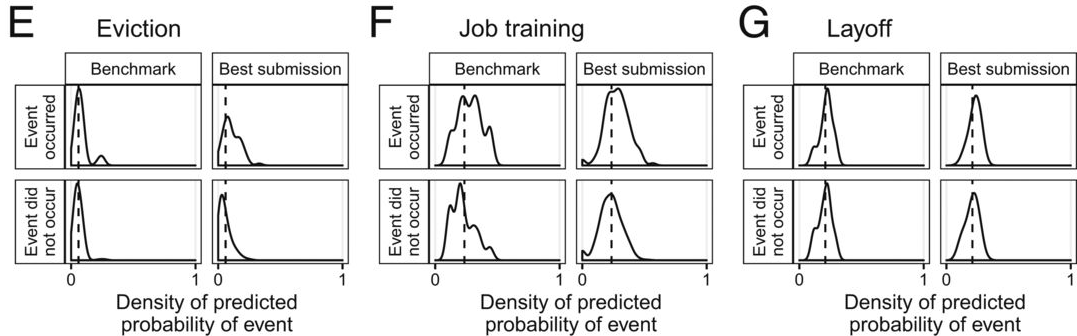
\includegraphics[width=0.9\textwidth]{figures/salganik_measuring_2020_fig3eg}} %
\end{center}

\vfill
Fig 3, \href{https://doi.org/10.1073/pnas.1915006117}{Salganik et al.\ (2020)}

\end{frame}
%%%%%%%%%%%%%%%%%%%%%%%%%%%
\begin{frame}

\begin{center}
\Large{What can we learn looking at all the predictions?}
\end{center}

\end{frame}
%%%%%%%%%%%%%%%%%%%
\begin{frame}

\begin{center}
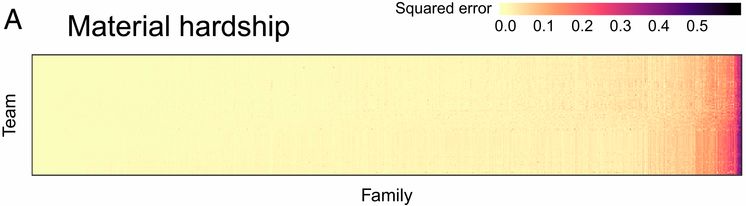
\includegraphics[width=0.90\textwidth]{figures/salganik_measuring_2020_fig4a}
\end{center}

\vfill
Fig 4, \href{https://doi.org/10.1073/pnas.1915006117}{Salganik et al.\ (2020)}
\end{frame}
%%%%%%%%%%%%%%%%%%%%%%%%%%
\begin{frame}


\begin{center}
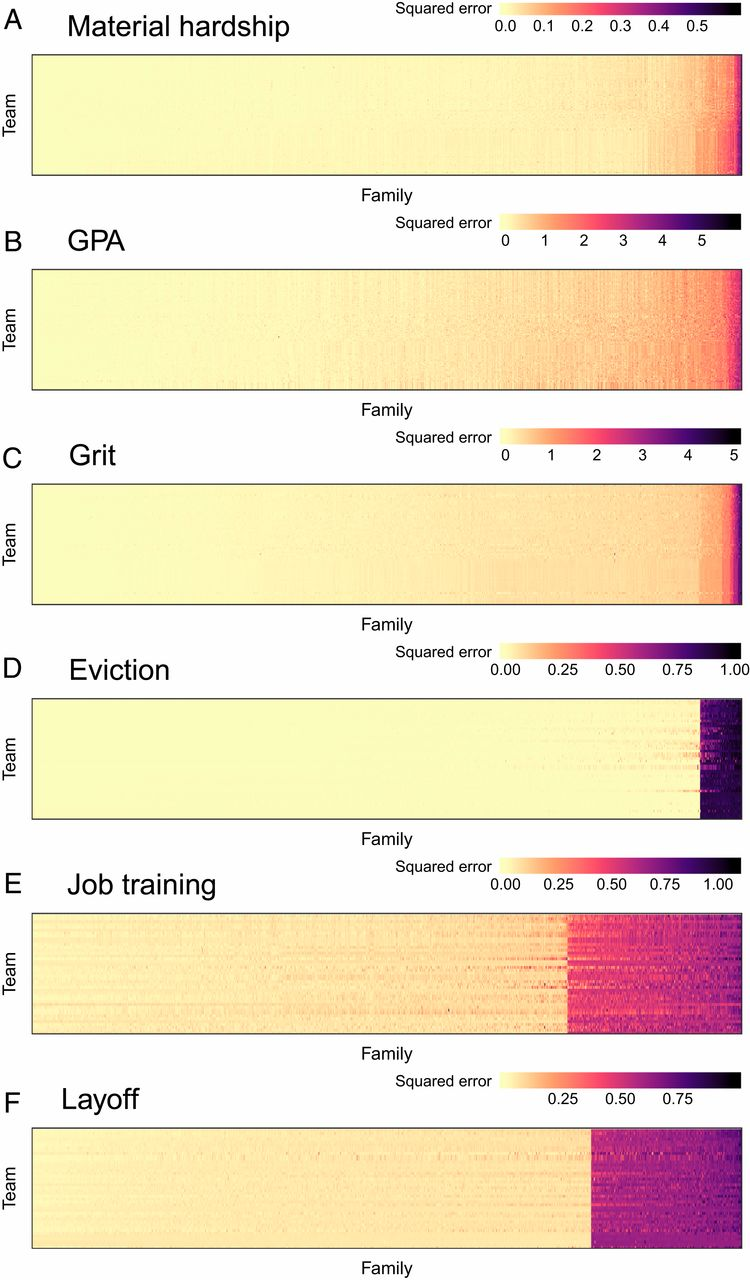
\includegraphics[height=0.90\textheight]{figures/salganik_measuring_2020_fig4}
\end{center}

\vfill
Fig 4, \href{https://doi.org/10.1073/pnas.1915006117}{Salganik et al.\ (2020)}
\end{frame}
%%%%%%%%%%%%%%%%%%%%%%%%%%
\begin{frame}

\begin{center}
\Large{What do these results mean for policy makers?}
\end{center}

\end{frame}
%%%%%%%%%%%%%%%%%%%%%%%%%%%%
\begin{frame}

\begin{itemize}
\item Machine learning is not magic\pause
\item Transparent evaluation of any algorithm is needed \pause
\item Complex models may not outperform simple models
\end{itemize}

\end{frame}
%%%%%%%%%%%%%%%%%%%%%%%%%%%%
\begin{frame}

\begin{center}
\Large{What do these results mean for researchers?}
\end{center}

\end{frame}
%%%%%%%%%%%%%%%%%%%%%%%%%%%%
\begin{frame}

Researchers must reconcile an ``understanding/prediction'' paradox \pause
\begin{itemize}
\item We don't understand much \pause
\item Prediction is not a good measure of understanding \pause
\item Our current understanding is correct but incomplete
\end{itemize}

\end{frame}
%%%%%%%%%%%%%%%%%%%%%%%%%%%%
\begin{frame}

\begin{center}
{\Large How can we expand our understanding?}\\ 
\vspace{0.5in}
\pause
{\Large In-depth, semi-structured interviews}
\end{center}

\vfill
Dark matter interview team: Rachel M. Brown-Weinstock, Bobbi Brashear, Kristin Catena, Susan Clampet-Lundquist, Sophie Damas, Katie Donnalley, Kaitlin Edin-Nelson, Kathryn Edin, Alexus Fraser, Sarah Gold, Ashley Hyman, Daniel Kim, Ian Lundberg, Abigail MacLean, Collin ``Ren'' MacLean, Stefanie Mavronis, Timothy Nelson, Matthew Salganik, Naomi Shifrin, and Vicki Yang.
\end{frame}
%%%%%%%%%%%%%%%%%%%%%%%%%%%
\begin{frame}

\begin{center}
\includegraphics[width=\textwidth]{figures/kaizen_cycle}
\end{center}

\end{frame}
%%%%%%%%%%%%%%%%%%%%%%%%%%%
\begin{frame}

\begin{center}
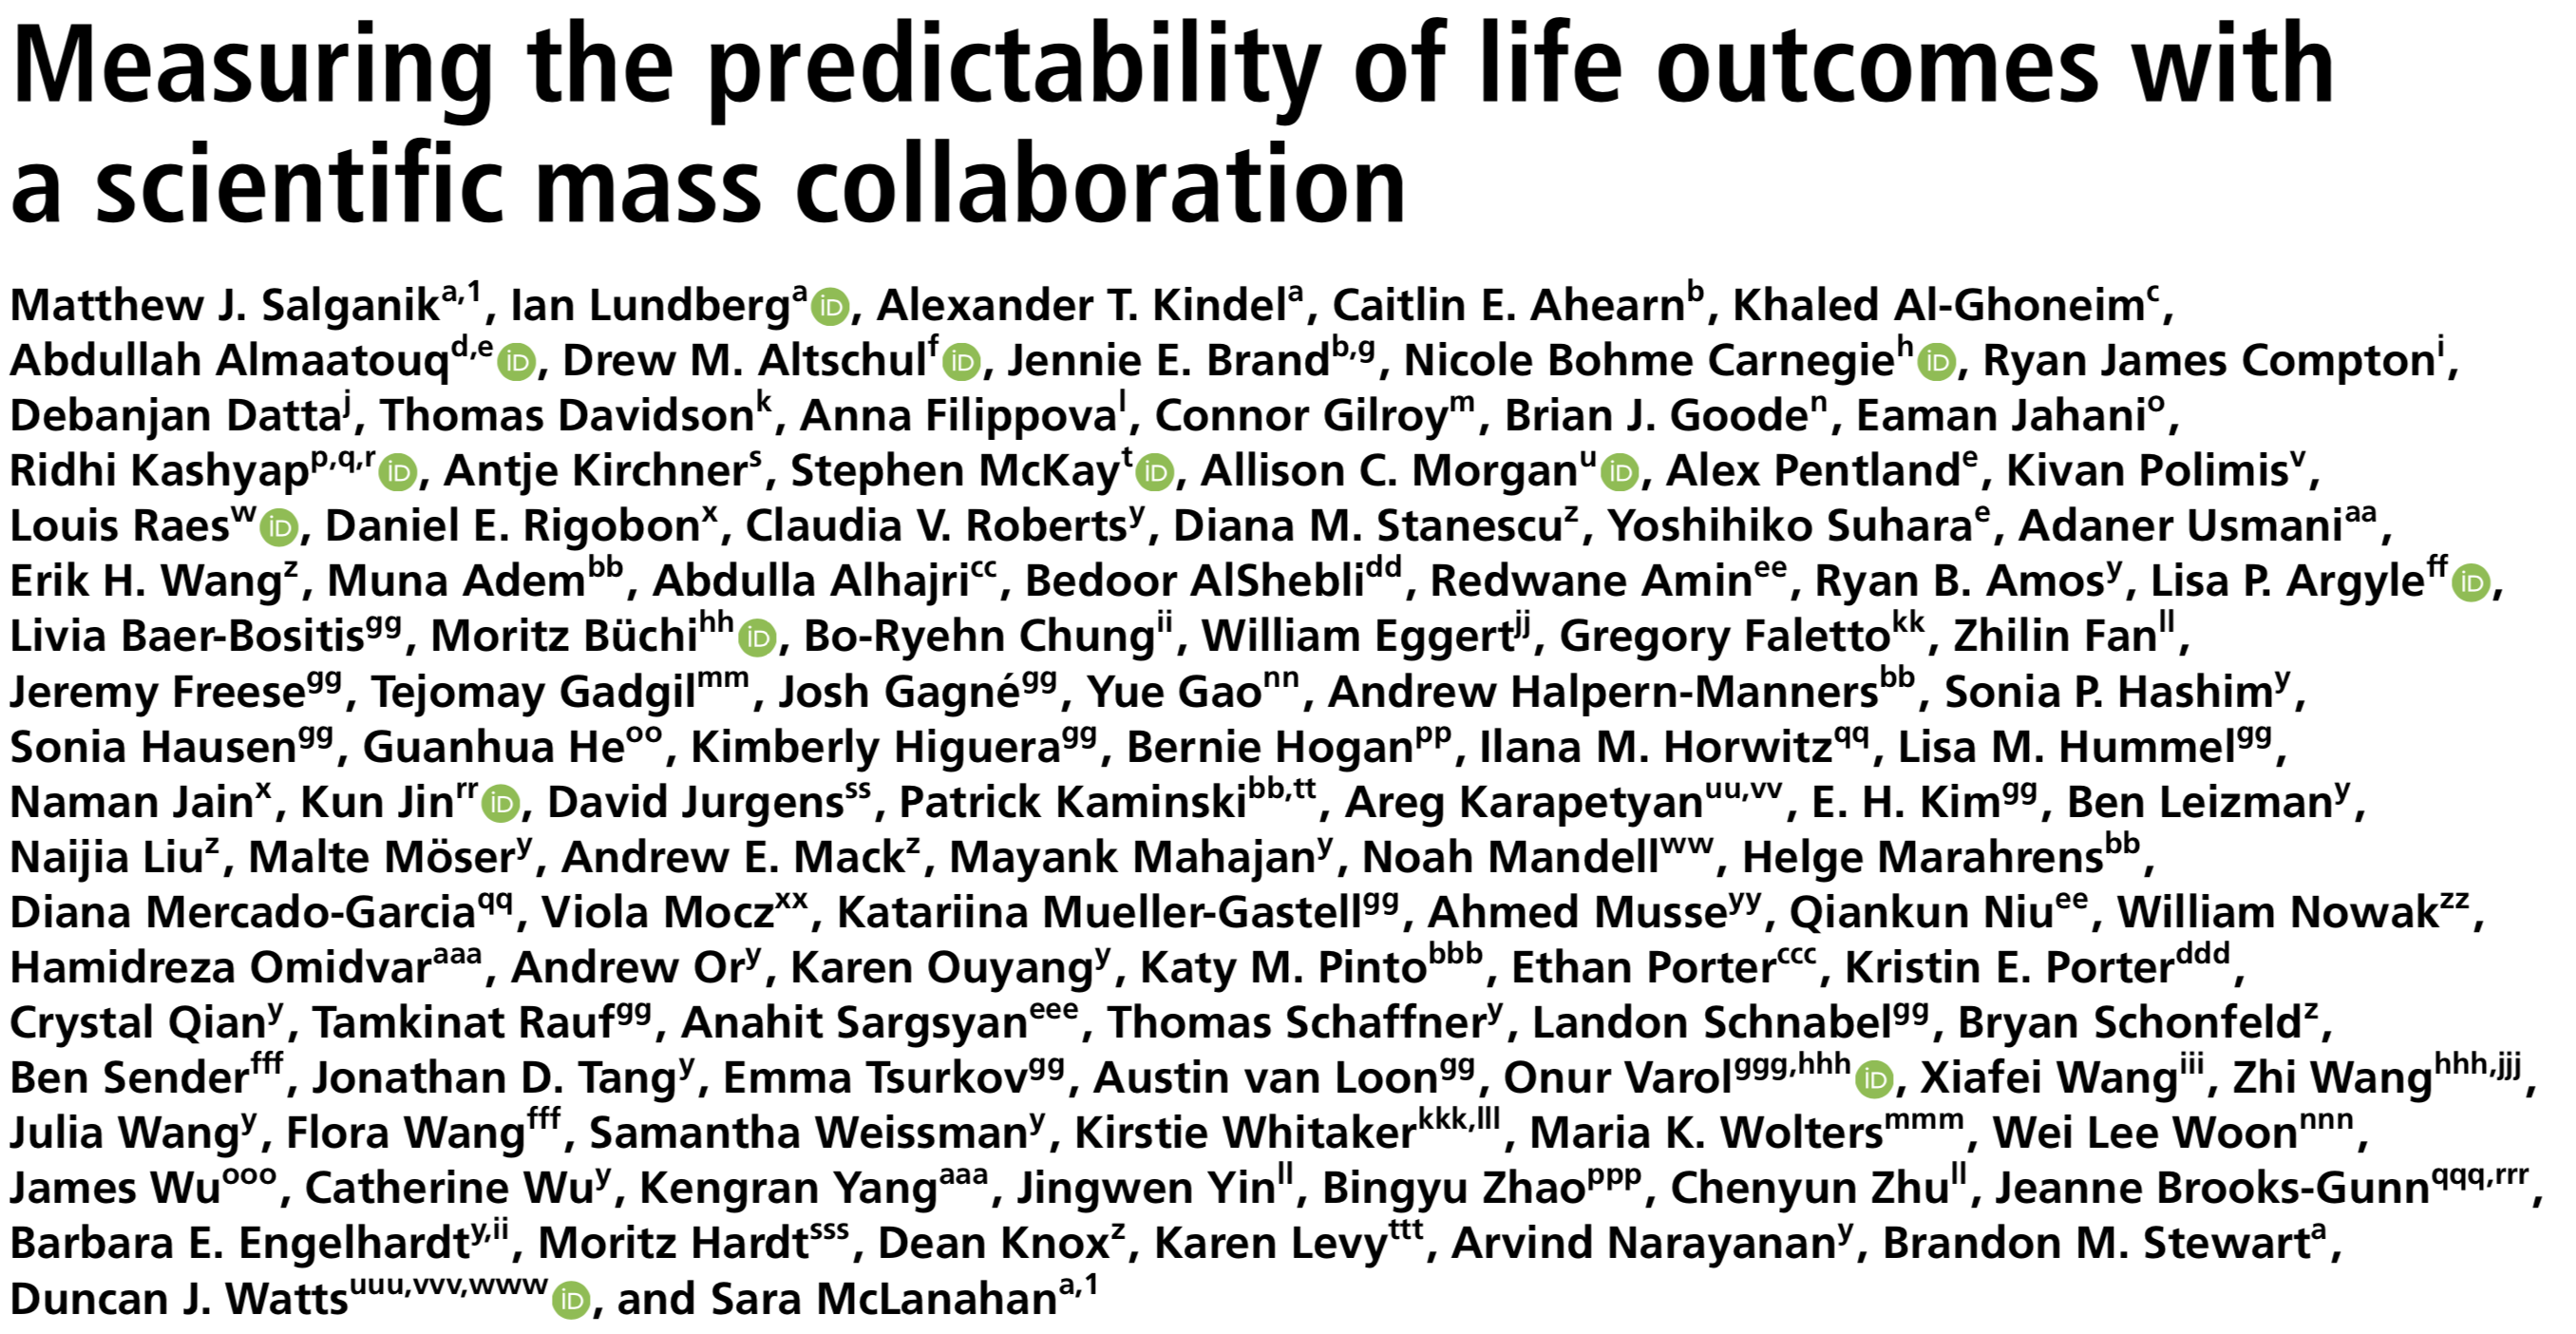
\includegraphics[width=0.9\textwidth]{figures/salganik_measuring_2020_title_authors}
\end{center}

\vfill
\url{https://doi.org/10.1073/pnas.1915006117}\\
See also Garip (2020) ``What failure to predict life outcomes can teach us'' \url{https://doi.org/10.1073/pnas.2003390117}

\end{frame}
%%%%%%%%%%%%%%%%%%%%%%%%%%%
\begin{frame}

\href{https://journals.sagepub.com/topic/collections-srd/srd-1-fragile_families/srd}{Special Collection of \textit{Socius} about the Fragile Families Challenge}
\begin{itemize}
\item 12 submitted manuscripts from Challenge participants (all with accompanying code and computing environment) \pause
\item 3 papers from our group \pause
\begin{itemize}
\item ``\href{https://doi.org/10.1177/2378023118813023}{Privacy, ethics, and data access: A case study of the Fragile Families Challenge}'' by Lundberg, Narayanan, Levy, \& Salganik \pause
\item ``\href{https://doi.org/10.1177/2378023118817378}{Improving metadata infrastructure for complex surveys: Insights from the Fragile Families Challenge}'' by Kindel, Catena, Hartshorne, Jaeger, Koffman, McLanahan, Phillips, Rouhani, Vinh, \& Salganik \pause
\item ``\href{https://doi.org/10.1177/2378023119849803}{Successes and struggles with computational reproducibility in the Fragile Families Challenge}'' by Liu \& Salganik
\end{itemize}
\end{itemize}

\end{frame}
%%%%%%%%%%%%%%%%%%%%%%%%%%%
\begin{frame}

\begin{center}
\LARGE{
$ \hat{y} \quad \& \quad \hat{\beta}$
}
\end{center}

\vfill
\href{https://dx.doi.org/10.1257/jep.31.2.87}{Mullainathan and Spiess (2017)}
\end{frame}
%%%%%%%%%%%%%%%%%%%%%%%%%%
\begin{frame}

\begin{center}
\includegraphics[width=0.6\textwidth]{figures/wikipedia_logo}
\end{center}

\end{frame}
%%%%%%%%%%%%%%%%%%%%%%%%%%
\title[]{\textcolor{gray}{[Introduction to mass collaboration], [Human computation], [Open call], [Distributed data collection],} \newline [Fragile Families Challenge]}
\author[]{Matthew J. Salganik\\Department of Sociology\\Princeton University}
\date[]{%Summer Institutes in Computational Social Science\\2020
%\vfill
%\begin{flushleft}
%{\scriptsize
%The Summer Institutes in Computational Social Science is supported by grants from the Russell Sage Foundation and the Alfred P. Sloan Foundation.}
%\end{flushleft}
\begin{flushright}

\includegraphics[width=0.1\textwidth]{figures/cc-by.png}
\end{flushright}
}
%%%%%%%%%%%%%%%%%%%%%%%%%
\frame{\titlepage}
%%%%%%%%%%%%%%%%%%%%%%%%%%
\end{document}

